\tableofcontents
\newpage
\baselineskip=18pt
\section{Introduction}
\setlength{\parindent}{5ex}
Traditionnellement, la mémoire partagée et la transmission de messages ont été les deux modèles de programmation pour la communication interprocessus et la synchronisation dans les calculs effectués sur un système distribué. La transmission de messages a été le moyen préféré pour gérer la communication interprocessus dans les systèmes multiprocesseurs faiblement couplés\footnote{Dans les systèmes faiblement couplés, chaque processeur possède sa propre mémoire locale, un ensemble de périphériques d’entrée-sortie et un commutateur de canal et d’arbitre (CAS)}, car les ordinateurs formant un système distribué ne partagent pas de mémoire physique. Le modèle de transmission de messages est caractérisé par le mouvement des données entre les
processus lorsqu'ils communiquent et se synchronisent en envoyant et en recevant des messages. En revanche, les systèmes multiprocesseurs étroitement couplés\footnote{Le système à couplage étroit comprend des processeurs, des modules de mémoire partagée et des canaux d’entrée/sortie} utilisent principalement le modèle de mémoire partagée car il fournit un support direct pour le partage des données.\par
Ces dernières années, les chercheurs ont exploité le paradigme de la mémoire partagée. Ils ont étudié son applicabilité aux systèmes faiblement couplés. Ces efforts ont abouti à l'introduction d'un nouveau concept qui combine le meilleur des deux modèles de base. Ce concept, communément appelé Mémoire Partagée Distribuée (DSM : Distributed Shared Memory), fait référence à l'abstraction de la mémoire répartie sur plusieurs systèmes, ainsi
donnant l'illusion d'une grande mémoire « partagée ». Comme l'illustre la figure 1, cette mémoire globale
s'étend sur les mémoires privées des processeurs composants et s'étend au-delà des limites de la machine.\par
DSM permet aux processus s'exécutant sur différents processeurs interconnectés de partager la mémoire en masquant le(s) emplacement(s) physique(s) des données, rendant l'emplacement mémoire transparent pour l'ensemble du système. Un avantage important de cette approche est que les programmes parallèles développés pour la mémoire partagée (réelle)
les systèmes peuvent s'exécuter sur des architectures distribuées sans aucune modification.\par
L'objectif ce projet est de mettre en place le logiciel DSM permettant de partager de la mémoire virtuelle entre plusieurs processus répartis sur différentes machines physiques.
\begin{figure}[H]
     \centering
     \begin{subfigure}[H]{0.9\textwidth}
         \centering
         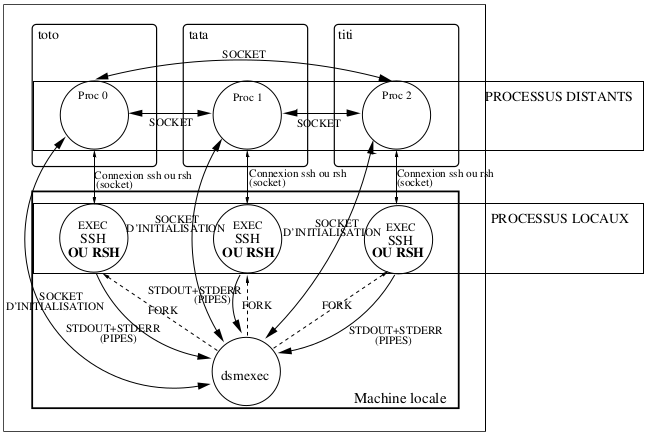
\includegraphics[width=\textwidth]{Archi.png}
     \end{subfigure}
     \caption{Architecture [1]}
\end{figure}

\newpage
\section{Phase 1 : Lancement des processus}
\setlength{\parindent}{5ex}
L'objectif de cette phase est de développer le programme $dsmexec.c$ qui a un rôle très important. Ce programme servira à lancer les processus de la DSM sur les différentes machines.

\subsection{Fonction et capacité du lanceur \texttt{dsmexec}}
\setlength{\parindent}{5ex}
Ce programme va avoir comme argument :\\
- Un fichier nommé \texttt{machine\_file} contenant les noms des machines concernées. On utilisera ce fichier pour avoir le nombre de processus qui sera égale au nombre d'entrées dans le fichier à l'aide de la fonction \texttt{read\_machine\_names} qui va au même temps stocker les noms dans une structure \texttt{dsm\_proc\_t} et compter le nombre des processus.\\
- Un nom d'un programme exécutable qui utilisera la DSM, et ses arguments.\\
Ainsi l'utilisateur va pouvoir lancer le logiciel avec la commande suivante :
\begin{center}
    \fbox{\texttt{dsmexec machinefile programme\_exécutable arg1 arg2 arg3...}}
\end{center} \\
\setlength{\parindent}{5ex}

\subsection{Fonction du programme \texttt{dsmwrap} et sa connexion avec \texttt{dsmwrap}}
Après la création des processus distants (avec ssh) à travers des processus fils en utilisant la fonction \texttt{execvp} pour l'exécution de la commande : \\
\fbox{\texttt{ssh nom\_machine dsmwrap dsmexec\_hostname dsmexec\_port pid truc arg1 arg2 arg3...}}\\ \\
Le programme intermédiaire, appelé \texttt{dsmwrap}, dont le rôle
consiste à “nettoyer” la ligne de commande avant d’exécuter la bonne commande, va permettre d'envoyer en premier lieu les informations concernant chaque machine (nom de la machine, pid, numéro de port). Après, le processus \texttt{dsmwrap} va créer une socket d'écoute pour les connexions avec les autres processus dsm, sa valeur avec la valeur de la socket de connexion avec \texttt{dsmexec} seront définis comme variables d'environnement respectivement avec \texttt{MASTER\_FD}  et \texttt{DSMEXEC\_FD} en utilisant la fonction \texttt{setenv} pour éviter de polluer les arguments du programme exécutable.  
\\ \par 
Le programme  \texttt{dsmexec} de sa part sera chargé d’envoyer les données nécessaires pour les connexions à tous les processus distants (nombre des processus distants, son rang, un nombre de structures de type \texttt{dsm\_proc\_conn\_t} égal au nombre total de processus distants), et cela via un protocole d'échange déterminé.\\\par

Ensuite, \texttt{dsmexec} va passer son temps à attendre que des données arrivent sur les tubes dédiés aux événements sur stdout et stderr en utlisant la fonction \texttt{read\_from\_pipe}.


\section{Phase 2 : Création de la bibliothèque DSM}

\setlength{\parindent}{5ex}

L'objectif de cette phase est de mettre en place la bibliothèque de DSM après avoir le lanceur \texttt{dsmexec} opérationnel. Cette bibliothèque contiendra deux fonctions \texttt{dsm\_init} et \texttt{dsm\_finalize}.

\subsection{ La fonction dsm\_init}
\setlength{\parindent}{5ex}

La fonction \texttt{dsm\_init} renvoie un pointeur : c’est le pointeur marquant le début de la zone de mémoire distribuée.
\begin{center}
    \fbox{\texttt{char *dsm\_init(int argc, char **argv)}}
\end{center}

\subsubsection{Initialisation des connexions avec les autres processus}
\setlength{\parindent}{5ex}
Cette fonction commence d'abord par la récupération des variables d'environnement pour que chaque processus distant récupère les informations envoyées par le lanceur, les informations de connexion des autres processus sont stockées dans un tableau nommé \texttt{proc\_conn\_info} de type \texttt{dsm\_proc\_conn\_t}.\\
Après, c'est l'étape d'initialisation des connexions avec les autres processus : connect/accept. La subtilité dans cette étape est de pouvoir éviter que chacun des deux processus distants attend l'acceptation de connexion de l'autre ( double socket pour une connexion) ce qui va bloquer le programme. C'est pour cela le protocole des connect/accept sera implémenté de la manière suivante : on accepte les connexions des autres processus dsm de rang inférieur et on se connecte avec les autres processus dsm de rang supérieur comme le montre la figure 2 avec les flèches de connections .
\begin{figure}[H]
     \centering
     \begin{subfigure}[H]{0.9\textwidth}
         \centering
         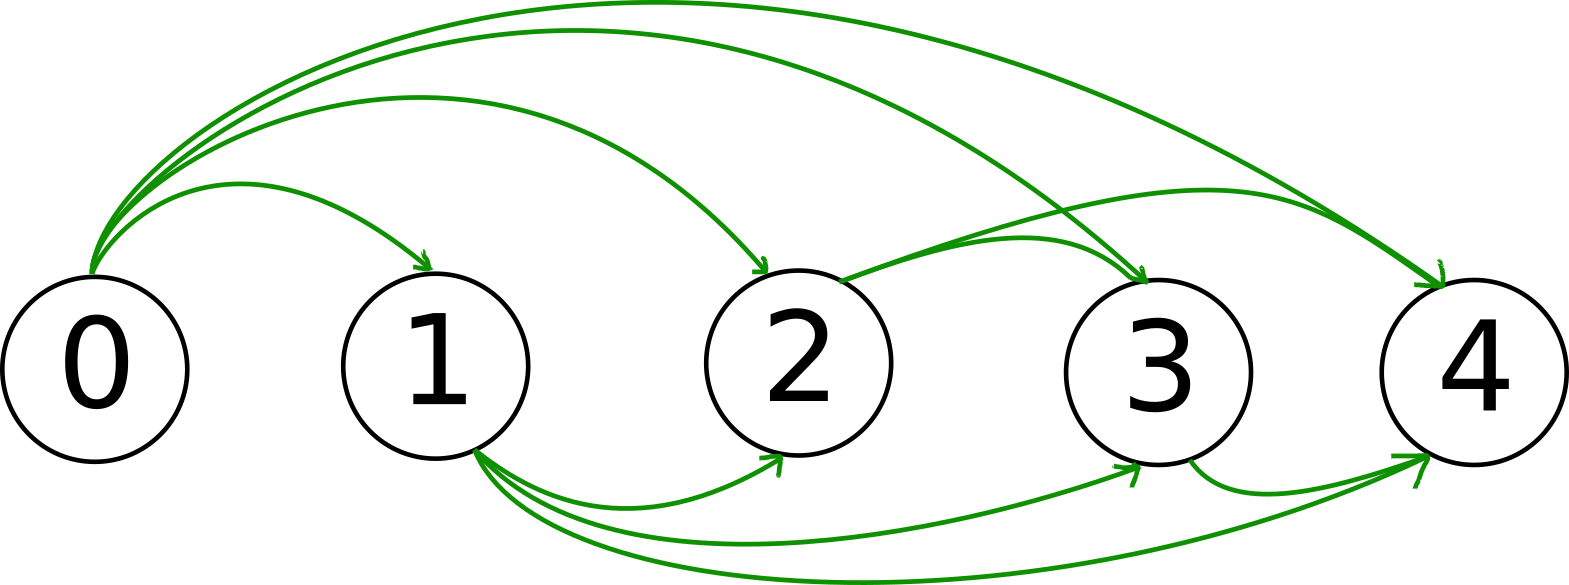
\includegraphics[width=\textwidth]{connect_accept.png}
     \end{subfigure}
     \caption{Connections de 5 processus distants}
\end{figure}


\subsubsection{Allocation des pages en tourniquet }
\setlength{\parindent}{5ex}
Chaque processus dispose d’une table \texttt{table\_page} où sont stockées des informations sur les pages mémoire :
propriétaire de la page, état de la page le cas échéant.\\
Pendant cette étape l’allocation des pages est faite cycliquement (figure 3), et la plage des adresses dans laquelle on travaillera sera comprise entre \texttt{BASE\_ADDR} et \texttt{TOP\_ADDR}. Cette plage d’adresses est identique pour l’ensemble des processus. Pour cela on va procéder à l'allocation que si le rang du processus est égale au reste de la division du numéro de page avec le nombre total des processus :
\begin{center}
    \texttt{Index}\%\texttt{DSM\_NODE\_NUM} = \texttt{DSM\_NODE\_ID}
\end{center}

\begin{figure}[H]
     \centering
     \begin{subfigure}[H]{0.9\textwidth}
         \centering
         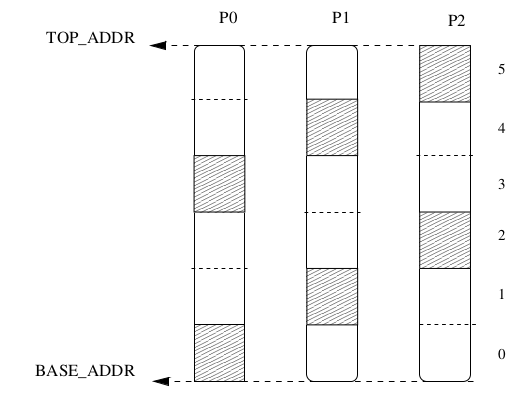
\includegraphics[width=\textwidth]{alloc.png}
     \end{subfigure}
     \caption{Répartition des pages [1]}
\end{figure}

\subsubsection{Mise en place du traitant de SIGSEGV et le flux de communication}
\setlength{\parindent}{5ex}
Dans le programme exécutable $exemple.c$, il se peut qu'un processus distant essaie de lire dans une plage d'adresses déjà allouée par un autre processus. Dans ce cas il reçoit un signal de type SIGSEGV qu'on devra s'assurer qu'il s'est passée entre \texttt{BASE\_ADDR} et \texttt{TOP\_ADDR} afin de le différencier d'un SIGSEGV normal.\\
Après c'est la fonction \texttt{dsm\_handler} qui va gérer la demande de cette page au propriétaire. Quant à la réception de la page, elle sera géré par son flux d'exécution \texttt{comm\_deamon} ce qui implique une synchronisation entre les deux flux.\\
Le protocole d'échanges des requêtes  est décrit par la figure suivante : 
\begin{figure}[H]
     \centering
     \begin{subfigure}[H]{0.9\textwidth}
         \centering
         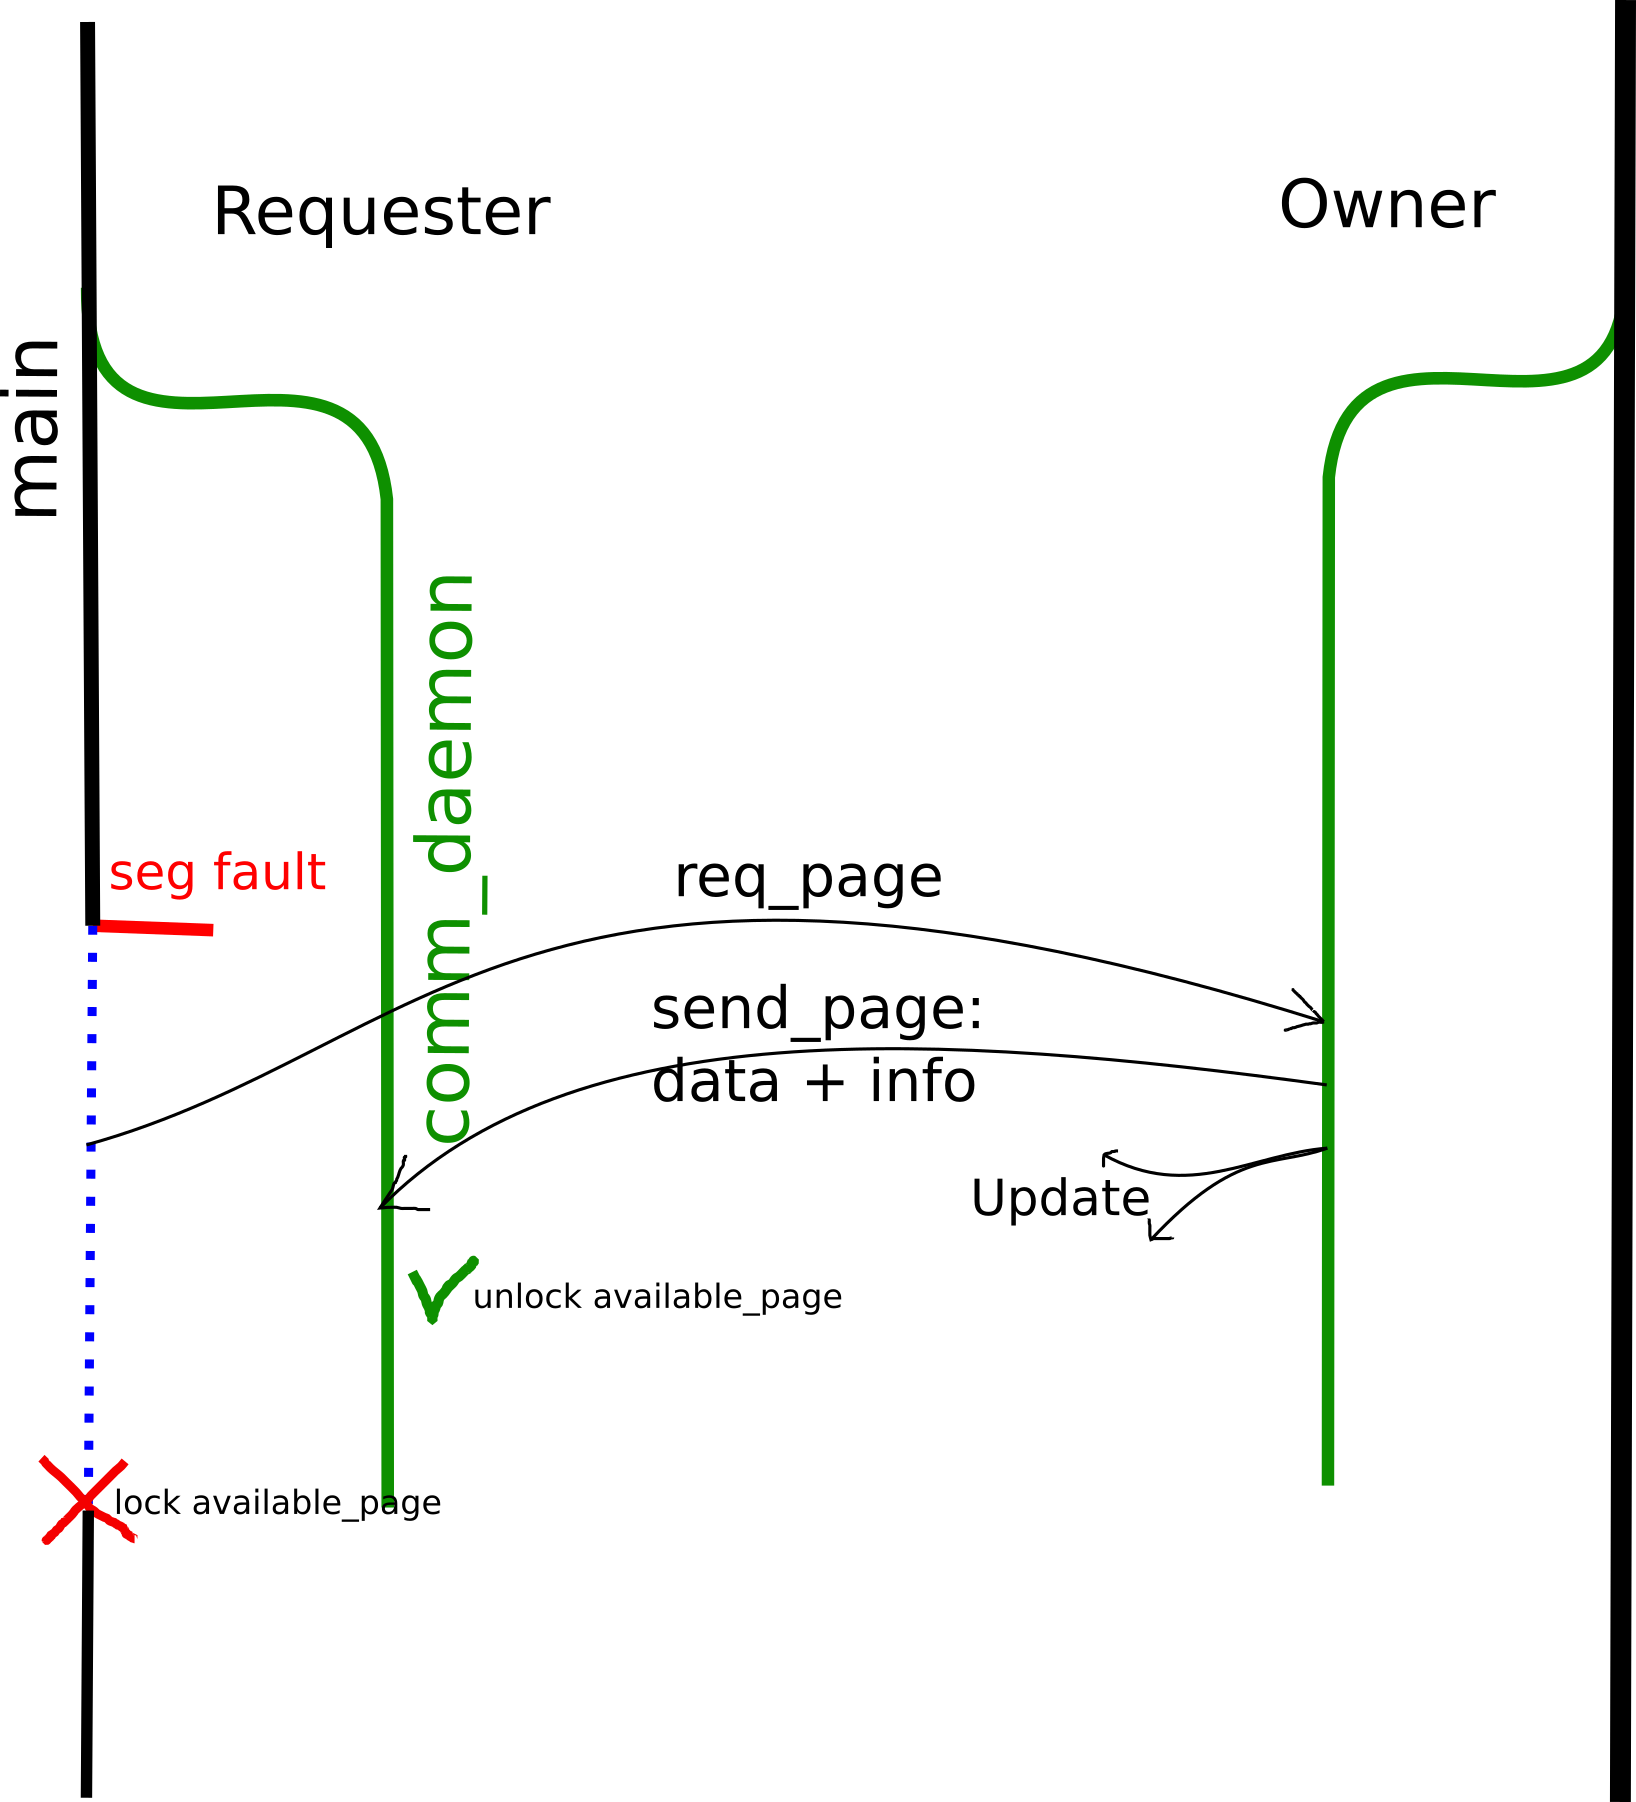
\includegraphics[width=\textwidth]{protocol.png}
     \end{subfigure}
     \caption{Protocole d'échange des requêtes}
\end{figure}
\noindent
Explication du protocole : \\
1- On stocke le numéro de la page demandée dans une variable accessible par le \texttt{comm\_deamon} pour vérifier lors de la réception de la page que c'est bien la page demandée (l'accès atomique est assuré par le mutex  \texttt{requested\_page\_mutex}).\\
2- On envoi la demande de la page avec un message de type \texttt{DSM\_REQ} en utilisant la fonction \texttt{dsm\_send}, la détermination de la socket convenable est assuré par la fonction \texttt{conn\_info\_get\_index\_by\_rank} qui retourne l'indice associé au rang dans le tableau \texttt{proc\_conn\_info}.\\
3- L'attente de la page est assurée par le mutex \texttt{available\_page}.\\
4- Le \texttt{comm\_deamon} du propriétaire reçoit le message de type \texttt{DSM\_REQ} et vérifie s'il est bien le propriétaire de la page, sinon il ne fait rien. Du coup le demandeur restera bloqué jusqu'à ce que son \texttt{comm\_deamon} reçoit un message de type \texttt{DSM\_UPDATE} qui va déverrouiller le mutex et donnera ainsi une nouvelle chance au demandeur (une nouvelle SIGSEGV). Si le demandeur reçoit une mise à jour concernant sa propre page il ne l'accepte pas ! car le message de type \texttt{DSM\_UPDATE} peut avoir un retard d'arrivée après une nouvelle mise à jour. \\
5- Le \texttt{comm\_deamon} envoie par la suite un en-tête (header) contenant le type du message (\texttt{DSM\_REQ}),le numéro de la page pour la vérification de l'étape 1, puis le message contenant les informations de la page et l'adresse de la page.\\
6- Le \texttt{comm\_deamon} met à jour sa \texttt{table\_page}, libère la page avec la fonction \texttt{dsm\_free\_page} et envoie aux autres processus les nouvelles modifications avec un message de type \texttt{DSM\_UPDATE}.\\
7- Le \texttt{comm\_deamon} du demandeur définit la variable \texttt{receiving\_timeout} dans le cas où il ne reçoit pas la page demandée pour des raisons divers. C'est pour cela à chaque fois que la variable \texttt{receiving\_time\_counter} atteint \texttt{receiving\_timeout} on déverrouille le mutex \texttt{available\_page} et on essaie une nouvelle fois d'envoyer la demande de la page pour éviter le blocage. Ce phénomène de blocage est remarqué lors de la réalisation d'un test exhaustif avec la commande suivante :
\begin{center}
    \fbox{\texttt{ while echo "----";do dsmexec machine\_file exemple; sleep 1; done;}}
\end{center} \\
en utilisant le programme exécutable exemple.c suivant :\\

\begin{lstlisting}[style=CStyle]
#include "dsm.h"
int main(int argc, char **argv)
{
  char *pointer;
  pointer = dsm_init(argc,argv);
  *((int *) (pointer + DSM_NODE_ID*sizeof(int))) = DSM_NODE_ID+100;
  
  for(int i = 0; i < DSM_NODE_NUM; i++){
    printf("%i | %i\n", i, *((int *) (pointer + i*sizeof(int))));
  }
  *((int *) (pointer + DSM_NODE_ID*sizeof(int))) = DSM_NODE_ID+200;
  
  for(int i = 0; i < DSM_NODE_NUM; i++){
    printf("%i | %i\n", i, *((int *) (pointer + i*sizeof(int))));
  }
  dsm_finalize();
  return 0;
}
\end{lstlisting}\newpage




\subsection{ La fonction dsm\_finalize}
\begin{center}
    \fbox{\texttt{void dsm\_finalize( void )}}
\end{center}
\setlength{\parindent}{5ex}

\texttt{dsm\_finalize} est censée s'exécuter à la fin des programmes qui utilisent le standard DSM. Son rôle est d'empêcher les processus de se terminer tant qu'il y a d'autres qui sont encore en train de s'exécuter. Cela assure la disponibilité des pages jusqu'à ce que le dernier processus termine son exécution.\\ Pour cela, dès qu'un processus arrive à la fonction \texttt{dsm\_finalize}, il envoie des requêtes de type \texttt{DSM\_FINALIZE} à tous les autres processus. Ensuite le \texttt{comm\_deamon} décrémente le nombre des processus actifs. Lorsque ce nombre atteint le zéro, il ne reste qu' à vérifier si le flux principal a terminé son exécution à l'aide de la variable globale \texttt{char finalize} (accés protégé par un mutex). Si les deux conditions sont vérifiées, le \texttt{comm\_deamon} se termine, le main fait un join et par la suite ferme les sockets, détruit les mutexes et libère la mémoire allouée.

\subsection{ Accès Atomique aux pages}
Parmi, les fonctionnalités que nous avons jugé primordiales que bonus c’était d’offrir à l' utilisateur des fonctions capables de synchroniser l'accès aux pages. Nous les avons imaginées avec les prototypes suivants:
\begin{lstlisting}[style=CStyle]
    Void unlockpage(int page_num);
    Void lockpage(int page_num);
\end{lstlisting}

Ce mécanisme empêche le \texttt{comm\_deamon} d’envoyer la page jusqu'à ce que unlockpage soit appelée.
\newpage
\section{Conclusion}

\setlength{\parindent}{5ex}
Ce projet nous a bien permis d'appliquer les notions vu en cours de la programmation système et réseaux dans le contexte d'implémentation du logiciel DSM.
Pendant la réalisation de ce projet, nous étions face à beaucoup d'obstacles remarquables et non remarquables. Concernant la phase 1 nous avions l'impression que tout marchait bien puisque les tests qu'on a réalisé depuis nos machines par l'intermédiaire du ssh fonctionnait normalement, par contre après la fin de cette phase nous étions surpris que cela bloque pour certaines machines de l'école. La nouvelle chance lors de la première séance de la phase 2 pour revoir nos problèmes dans la phase 1 nous a permis de résoudre le blocage. En effet, l'utilisation de \texttt{bash -c} avant le ssh était la source du problème, son utilisation est justifiée par le faite que nos tests étaient toujours réalisés depuis nos machines locaux et les tests ne fonctionnaient que lorsqu'on l'ajoute avant la commande ssh pour créer les processus. \\
Concernant la phase 2, la difficulté consistait à établir un bon protocole pour éviter dans n'importe quel cas le blocage de notre programme. C'est pour cela nous avons testé avec un programme exécutable où tout les processus distants essaient de lire et écrire dans la même page simultanément. Ce qui nous a permis d'améliorer à chaque fois un protocole qui gère bien des cas critiques.\\
Enfin, nous avons eu le plaisir de réaliser ce genre de projet, car à chaque fois qu'un problème apparaît, c'est un nouveau défi pour nous de le résoudre ce qui nous a permis d'améliorer nos compétences dans la programmation système et réseaux.

\section{Référence}

[1] Sujet du projet.








